\section{Impact of Locality}
Locality is widely used in many deduplication solutions, e.g., Zhu et al.~\cite{bottleneck08}
put in memory cache of block indices near the one which result in a disk index look-up and is found.
This is base on the observation that duplicates usually come in sequence rather than independently.

We check this fact in VM snapshots by monitoring the modification locations in VOSS. 
For each snapshot, we compare it to the previous snapshot, in the unit of 2MB fix-sized page,
to find out locations of dirty pages since last backup. We end up with a bitmap of
dirty pages for every snapshot, except those earliest ones who don't have a previous version
to compare against.

\begin{figure*}[htb]
  \centering
  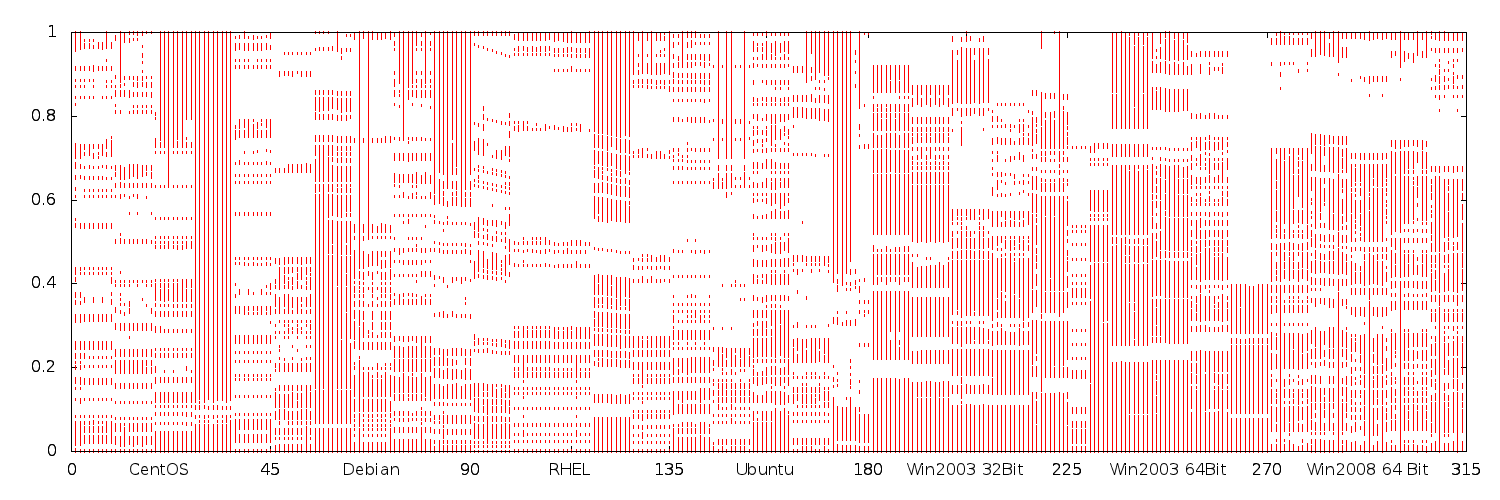
\includegraphics[width=6.5in,height=2in]{countmodify.png}
\caption{Bitmaps of dirty pages between snapshots}
\label{fig:dirty}
\end{figure*}

In Figure~\ref{fig:dirty}, a snapshot's bitmap of dirty pages is represented as a vertical line 
composed of discontinuous segments. 
For each vertical line, the solid segments indicate changed regions since last snapshot backup,
and the rest represent the unchanged part.
All page locations (offset) is normalized with respect to the virtual disk size.
Because the earliest snapshots are excluded, 
every VM has 9 lines and there are 45 lines from each OS.
The bitmaps are first grouped by VMs and then by their OS type,
borders between OS types are shown as numbers at the xtics.

\emph{Observation 4: Each VM do has its own specific interested write regions, as a result, 
unchanged regions appear to be large and continous.} We see almost all VMs have
their write regions aligned across 9 snapshots, leaving the unchanged regions aligned as well.
So duplicates in the white area do come together during snapshot backup.
This observation strongly proves the importance of locality as the primary indication of
finding duplication.

\emph{Observation 5: Windows tends to write to more disk locations than Linux.} 
Although there are several Linux VMs write to large area of disk locations, this is very likely
because those users were more active during our samlping period.
On the other hand, all Windows VMs write to almost everywhere of the disk during every backup period.
We believe this is due to the design difference between NTFS and ext3, and we also see
the upgrade from Win2003 to Win2008 reduces such writes. However, this doesn't mean windows has more 
dirty pages, it's just more scattered.


In order to see the impact of locality further, we investigate deeper into the dirty pages.
We split those fix-sized pages into variable-sized 4KB blocks, for every block in the dirty pages,
we look into the corresponding
page (base on offset) of previous snapshot to see if a duplicate can be found.

\begin{table}[htb]
  \centering
    \begin{tabular}{|l|p{1.3in}|p{0.4in}|}
        \hline
        OS Type & After Reduction Within \newline Dirty Page (GB) & Ratio \\ \hline
        Debian & 161.11 & 6.42 \\ \hline
        Ubuntu & 145.02 & 6.82 \\ \hline
        RHEL & 185.34 & 5.43 \\ \hline
        CentOS & 479.78 & 2.03 \\ \hline
        Win2003 32Bit & 80.14 & 7.87 \\ \hline
        Win2003 64Bit & 95.07 & 8.35 \\ \hline
        Win2008 64Bit & 172.22 & 9.76 \\ \hline
        Combined & 1318.68 & 5.26 \\
        \hline
    \end{tabular}
    \caption{Data reduction via 4KB block deduplication within dirty pages}
    \label{tab:locality}
\end{table}

\emph{Observarion 6: Data reduction ratio is generally improved, but there is still lots of
improvment space compare to complete deduplication.} We see significant improvment for all OS
types, which definitely deserves adding an additional layer to dirty-page based 
data reduction. In addition, the cost of looking one page's block hash index
shall be very small compare to full hash index lookup.

However, this is probably the best of what we can get from locality. The rest of
duplication mainly lies between VMs, e.g., same or slightly different versions of OS distributions, 
similar software installations, etc. Such duplications can not be easily 
eliminated and worth further research efforts.
